\chapter{Experiments}
\label{chap:4}
%

- parallel runs on the cluster
- BO : We set the initial sample count $M = 10$ and the iteration count $N = 200$.

\section{Implementation}

\subsection{Problem environment}
In early test runs we used \texttt{Matlab} implementations of cart pole, acrobot, and mountain car adapted from \cite{joseCode}. But later we implemented OpenAI Gym to have a wide range of problem environments available and to have consistent rewarding functions. Otherwise, the rewarding function would depend on the source and therefore produce less comparable results.



\subsection{Gaussian Process Regression}

(difference between full covariance and cov vector)

Instead of calculating the inverse of $K_n$ in \eqref{eq:meanGauss} we use the lower Cholesky decomposed matrix:

$$LL^\top=K_n$$

This is considered faster and numerically more stable \cite{rasmussen2006gaussian}. The mean vector $\mu$ is then computed as follows:

\begin{equation} \label{eq:regression}
    \mu = K_n^{-1}\,y = (L\,L^{T})^{-1}\,y = (L^{-T}\,L^{-1})\,y = L^{-T}\,(L^{-1}\,y) = L^{T}\setminus(L \setminus y).
\end{equation}

The backslash operator denotes the matrix left division, so the solution $x=A\setminus b$ satisfies the system of linear equations $A\,x=b$.
Matrix $K_n$ must be positive definite for the cholesky decomposition. So we double the noise variance hyperparameter $\sigma_n^2$ from \eqref{eq:kNoise} until positive definiteness is achieved.

For the expected improvement function we only need the vector of variances. Instead of calculating the whole covariance matrix $V$ we can take a shortcut. All elements on the diagonal of $K(X_*,X_*)$ equal $\sigma_f$ because the difference between one $x_*$ and the same $x_*$ is zero. Therefore we write:

$$L_k = L \setminus K(X_*,X)$$

$$v = \sigma_f - \sum_{\text{rows}} (L_k \circ L_k).$$

This adaptation is inspired by \cite{nandoCode} and reduces the computational effort drastically.

For the whole covariance matrix we also avoid calculating the matrix inverse:

$$V = K(X_*,X_*) - (L_k^\top L_k)^\top $$




\subsection{Action selection}

In continuous action space we use a linear policy to action mapping

$$a = f_s(s)^\top x + \epsilon_a,$$

with a small gaussian noise $\epsilon_a$ needed for stochastic policies. So the actions are Gaussian distributed:

$$a \sim \mathcal{N}(f_s(s) x,\epsilon_a^2).$$

In discrete action space environments we use a parametric soft-max action selection policy:

$$P(a|s)= \frac{\exp(f_s(s)^\top x_a)}{\sum_{i\in A} \exp(f_s(s)^\top x_i)}.$$

Again it consists of the linear mapping $f_s(s)^\top x$, and $A$ holds all possible actions. The resulting action is then sampled from the probability of action $a$ given state $s$.

The state feature function $f_s(s)$ is defined for each environment as shown below.

\section{Cart pole}


% \begin{figure}
%     \begin{center}
%         \fbox{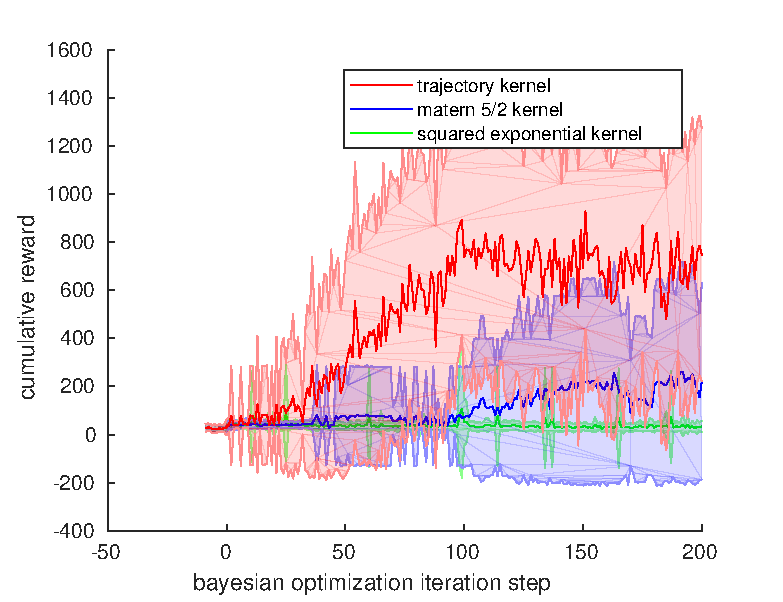
\includegraphics{/home/sebastian/Documents/bscThesis/img/cartpole_matlab_conti_oldreward.pdf}}
%         \caption{Global opt, 4 dim. Mean and standard deviation from 32 trials of each kernel. Cartpole matlab implementation with old reward function, 1000 timesteps, and continuous action selection.}
%     \end{center}
% \end{figure}
%
% \begin{figure}
%     \begin{center}
%         \fbox{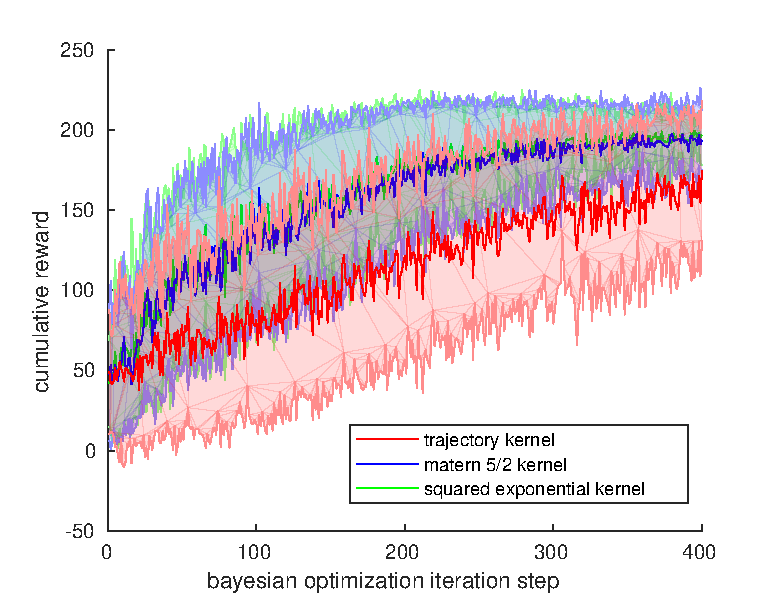
\includegraphics{/home/sebastian/Documents/bscThesis/img/cartpole_matlab_conti_newreward_local}}
%         \caption{Local opt, 4 dim. Mean and standard deviation from 32 trials of each kernel. Cartpole matlab implementation with new reward function, 200 timesteps, and continuous action selection.}
%     \end{center}
% \end{figure}
%
% \begin{figure}
%     \begin{center}
%         \fbox{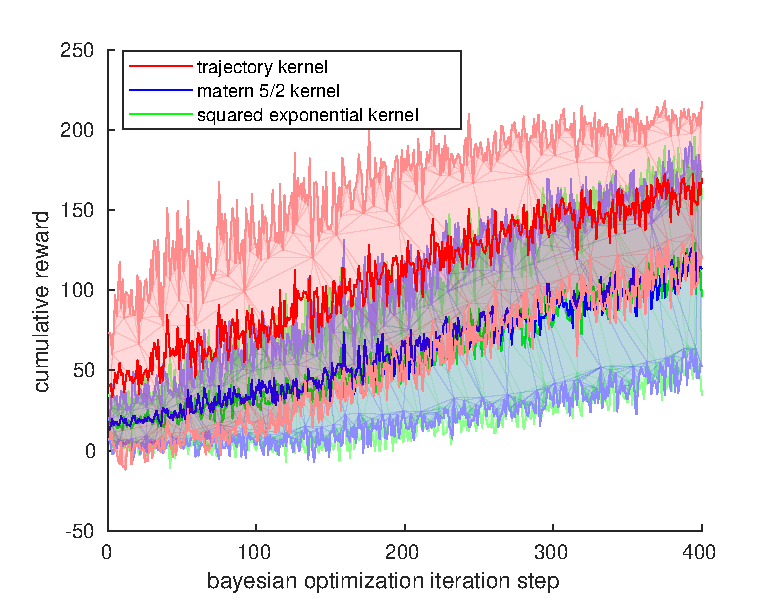
\includegraphics{/home/sebastian/Documents/bscThesis/img/cartpole_pygym_disc_local}}
%         \caption{Local opt, 10 dim. Mean and standard deviation from 32 trials of each kernel. Cartpole python gym implementation, 200 timesteps, and discrete action selection.}
%     \end{center}
% \end{figure}
